\cotefile{148}
\scanpage{10}

\noindent\begin{minipage}[t]{0.43\textwidth}
\centering
U N I V E R S I T E\\
DES SCIENCES ET TECHNIQUES\\
DU LANGUEDOC\\
\textasciicircum\textasciicircum\textasciicircum\textasciicircum\textasciicircum\textasciicircum\textasciicircum\textasciicircum\textasciicircum\textasciicircum\textasciicircum\textasciicircum\textasciicircum
\end{minipage}\hfill
\begin{minipage}[t]{0.49\textwidth}
\raggedleft
\vspace{1.5\baselineskip}
Montpellier, le 18 octobre 1983
\end{minipage}

Service de la Scolarité

Diffusion : Liste A\\
AM/gs \qquad N° 4570

\begin{center}
AVIS DE SOUTENANCE D'UNE THESE DE DOCTEUR-INGENIEUR

``ECOLOGIE GENERALE ET APPLIQUEE \quad option \quad ECOLOGIE TERRESTRE''

\texttt{============================================================}
\end{center}

\uline{NOM et prénom du candidat} : MOUFADDAL Mohamed

\uline{Titre de la thèse} : ``CONTRIBUTION A L'ETUDE DES POSSIBILITES D'EXTENSION\\
DU CEDRE DE L'ATLAS EN DEHORS DE SON AIRE ACTUELLE''

\uline{Date, heure et lieu de soutenance p\unsure{\deleted{\illegible{1}}}révus} : Le 28 octobre 1983 à 14 heures\\
à l'Institut de Botanique

\uline{Nom du directeur de thèse} : M. GODRON Michel

\uline{Désignation du laboratoire où la thèse est préparée} : Centre d'Etudes\\
Phytosociologiques et écologiques Louis Emberger (CNRS)

\uline{Aanlyse de l'ouvrage} : L'objet de cette étude étant de cerner les\\
possibilités d'extension du Cèdre (\uline{Cedrus atl\unsure{\deleted{\illegible{1}}}a}n\uline{tica} Manetti) en dehors de\\
son aire actuelle, il a fallu, après une analyse de l'histoire de répartition du\\
Cèdre, préciser les facteurs climatiques responsables de la distribution\\
actuelle.

Les régions où l'introduction du Cèdre est possible,\\
sont déterminées à partir de l'étude climatique de stations situées à l'intérieur\\
et à l'extérieur de l'aire du Cèdre, et par une étude écologique et dendromé-\\
trique comparative de quelques plantations.

\uline{Durée approximative des recherches ayant abouti à la thèse} : 5 ans

\uline{Composition du jury proposé} : \begin{tabular}[t]{ll}
MM. & GODRON M.\\
& BEDEL J.\\
& SCHOENENBERGER A.\\
& ROMANE F.\\
& DAGET Ph.
\end{tabular}

\begin{flushright}
P/ le Secrétaire Général,\\
l'Attachée principale d'administration\\
scolaire et universitaire,

% Signature: the alphabetic proposal A. Gentil remains undecided.
\unsure{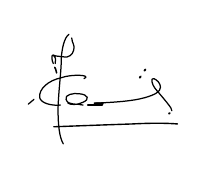
\begin{tikzpicture}[x=0.012cm,y=-0.012cm,line cap=round,line join=round,baseline=-0.4ex]
\draw[line width=0.45pt] (57,12) .. controls (52,16) and (50,26) .. (49,36)
  .. controls (49,52) and (46,71) .. (45.5,91)
  .. controls (45.5,109) and (47,121) .. (51,128);
\draw[line width=0.45pt] (60,16) .. controls (60,21) and (64,24) .. (62,29)
  .. controls (61,34) and (56,37) .. (52,36)
  -- (43,35) .. controls (41,33.8) and (39,33.5) .. (39,35)
  .. controls (39,39) and (39.5,42) .. (40.5,43)
  (41,35) .. controls (43,36) and (43.5,40) .. (42.5,43);
\draw[line width=0.55pt] (42,47) -- (43,49) -- (44,53);
\draw[line width=0.45pt] (73,59) .. controls (82,55) and (60,54) .. (49,58)
  .. controls (35,61) and (25,70) .. (26,79)
  .. controls (27,85) and (39,88) .. (48,87);
\draw[line width=0.45pt] (14,86) -- (20,81);
\draw[line width=0.45pt] (72,87) .. controls (66,85) and (56,88) .. (54,81)
  .. controls (52,76) and (62,74) .. (68,75)
  .. controls (78,76) and (79,81) .. (72,84)
  .. controls (66,87) and (59,87) .. (56,85);
\draw[line width=0.65pt] (77,87) -- (92,87) -- (93,85) -- (84,85);
\draw[line width=0.45pt] (85,85) .. controls (105,84) and (124,83) .. (138,79)
  .. controls (148,76) and (154,73) .. (154,68)
  .. controls (154,64) and (150,60) .. (147,59)
  .. controls (143,58) and (145,65) .. (148,69)
  .. controls (152,74) and (161,84) .. (165,90)
  -- (166,93);
\draw[line width=0.7pt] (132,58) -- (133,56.7);
\draw[line width=0.7pt] (137,50.6) -- (138,49.3);
\draw[line width=0.7pt] (163,96) -- (163.8,95.6);
\draw[line width=0.5pt] (41,110) .. controls (67,109) and (94,108) .. (124,107)
  .. controls (143,106) and (160,106) .. (172,107);
\end{tikzpicture}}

\uline{A. GENTIL}
\end{flushright}

\margin{9}

